
\section{Baseline Results}
\label{sec:baseline}

\subsection{Baseline: The 1-to-1 benchmark}

\newcommand{\configIntervalVsBaselineRatioQuantile}{q50}
\newcommand{\configIntervalVsBaselineRatio}[1]{\ptpKey{config/interval/#1/rpi-4/linuxptp/\configIntervalVsBaselineRatioQuantile}/\ptpKey{base/rpi-4/linuxptp/\configIntervalVsBaselineRatioQuantile}}

% good results for slow sample rate, bad ones for faster
\foreach \i in {-1,+0,+1,+2,+3}{
    \assertRange{\configIntervalVsBaselineRatio{\i}}{0.8}{1.2}
}
\foreach \i in {-2,-3,-4,-5,-6}{
    \assertRange{\configIntervalVsBaselineRatio{\i}}{1.2}{10}
}

We start by establishing a baseline for each tested system and vendor which we can later use as a comparison for different environment configurations. For each vendor, the default PTP/NTP profile is used as we expect this to be among the most widely deployed. We collect data in 20 minute runs (corresponding to just above 1000 samples per run), while retaining the default setting of one synchronization and one measurement of the path delay per second, as our results suggest that a higher frequency does not significantly improve clock synchronization (we observe the best synchronization quality results for LinuxPTP on the Raspberry-Pi 4 at 2 samples/second or slower) while it does negatively impact the stability of the measurement (for the highest rate setting -7, corresponding to \fpeval{1/(2^(-7))} samples/s, we observe a \fRatio{\configIntervalVsBaselineRatio{-7}} worse median accuracy and \renewcommand{\configIntervalVsBaselineRatioQuantile}{q95}\fRatio{\configIntervalVsBaselineRatio{-7}} at the 95\textsuperscript{th} percentile \PNineFive{}).

\begin{figure}
    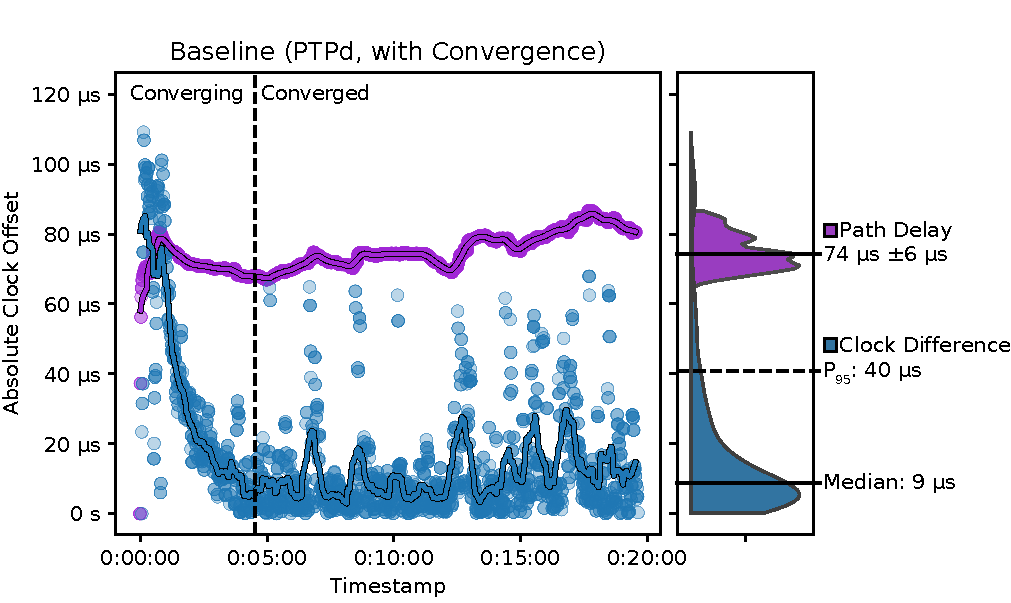
\includegraphics[width=\linewidth]{res/generated/base/rpi08-convergence_2.pdf}
    \caption{A sample run of PTPd in its default configuration (left: scattered raw signal and denoised moving average, right: kernel density estimates). Clock synchronization can follow different convergence trajectories, which needs to be accounted for when calculating statistics. Because PTP uses path delay compensation, the final clock synchronization accuracy is much better than the one-way path delay.}
    \label{fig:baseline_sample}
\end{figure}

Figure \ref{fig:baseline_sample} shows a sample run of the baseline for the PTPd vendor. In order to collect meaningful statistics, we apply some preprocessing to the collected profiles. The most important step is to remove the convergence phase (Figure \ref{fig:baseline_sample} left) from the profile to avoid it skewing the summary statistics, so that only the stable state is metricized. However, the clock travels on a different trajectory during each trial, and each convergence trajectory may take different amounts of time, have different final magnitudes, and include discontinuities, rebounds, and clock steps. To eliminate this unwanted data, we apply a heuristic to the raw clock offset: if the estimated offset repeatedly fluctuates between positive and negative, signifying that the local clock is ahead or behind the master, respectively, this implies that there is no clear pattern to the measured offsets that PTP can compensate for, and thus the clock offset is close to stable at its minimum value.
%Intuitively, this is somewhat equivalent to the average signed clock offset being zero, but note that the two are distinct for certain corner cases, as there are ways to produce an average zero clock offset that still exhibit a signal trend (which we want to avoid) and there can be large magnitude measurement outliers that cause a non-zero average clock offset while showing no trend.
%Empirically, we find that using the frequency of sign switches in the clock offset produces much more accurate predictions of whether a clock is synchronized than relying on average (signed) offset.
%\todo{@Arpan I commented out some data-processing discussion as you were marking it as confusing.}

% Note: This section contains a lot of data extracted by hand.
Separating the convergence phase from the stable phase is not only useful for calculating statistics, it also tells us how long we should wait after connecting to the master before we actually use the clock. Starting from an offset of 1 minute between the master and slave nodes before the clock step, we find that PTPd is by far the slowest vendor at establishing synchronization on all boards, on average taking 6 minutes to achieve stability on the Raspberry-Pi 5 but sometimes requiring 10 minutes or more, depending on how imprecise the initial clock step was. Just a 28\,ms offset after the clock step will cause around 13 minutes of clock slew with PTPd, whereas the other vendors can tolerate larger offsets in under 1 minute. LinuxPTP, SPTP and Chrony all convergence on average in under 1 minute across all boards (under non-degraded circumstances when the cluster is idling), with the longest baseline observation requiring 02:40 for LinuxPTP on TK1.

\cmpSearchVendor{\ptpKey{base/rpi-4/\vendor/pd/q50}/\ptpKey{base/rpi-4/\vendor/q50}}
From Figure \ref{fig:baseline_sample} we also observe that the clock offset is much lower than the corresponding path delay, due to the path delay compensation used by PTP clients. Across the tested vendors, we observe that the median absolute clock offset is between \fRatio{\cmpMin} (\fVendor{\cmpMinArg}) and \fRatio{\cmpMax} (\fVendor{\cmpMaxArg}) smaller than the magnitude of the path delay on the Raspberry-Pi 4 cluster,%
\cmpSearchVendor{\ptpKey{base/rpi-5/\vendor/pd/q50}/\ptpKey{base/rpi-5/\vendor/q50}}%
and \fRatio[-1]{\cmpMin} (\fVendor{\cmpMinArg}) to \fRatio[-1]{\cmpMax} (\fVendor{\cmpMaxArg}) smaller on the Raspberry-Pi 5 cluster, where hardware support is available.\todo{Arpan wants something to look at but so far we only provide text.}

Note that we show the \emph{absolute} clock difference, this represents the best estimate of the actual clock offset. It exhibits high skew due to the fact that the value cannot be negative, and the signal can experience bursts of noise which makes determining the true clock offset more difficult. While the actual offset estimate is useful, \PNineFive{} is more useful as a heuristic for the bound because packet delay variation as a source of noise generally dominates the actual clock drift -- using a high quantile can be thought of as a safety margin, but there is a tradeoff as last few percent are mostly noise leading to very high margins and lengthy testing required when using e.g. the maximum.

\subsection{Vendors \& Systems}

\begin{figure}
    \centering
    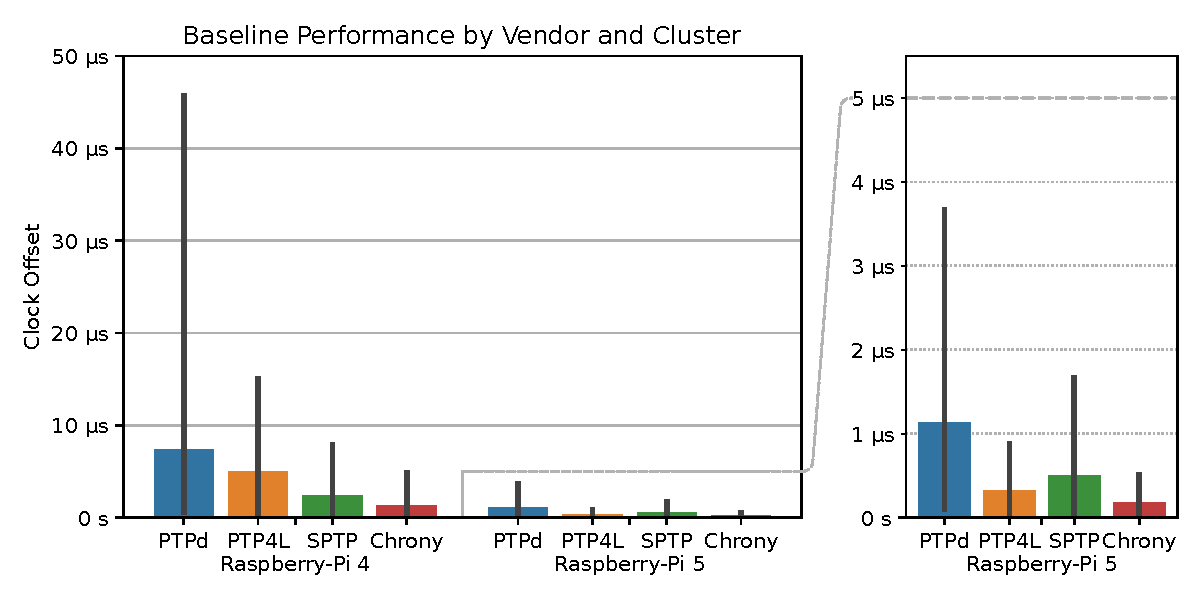
\includegraphics[width=\linewidth]{res/generated/base/vendor_comparison.pdf}
    \legend
    \caption{Median baseline performance for all vendors, across our two hardware testbeds (left) and magnified for only the Raspberry-Pi 5 cluster (right). Error bands represent \PFive{} and \PNineFive{}, respectively.}
    \label{fig:baseline}
\end{figure}

\begin{table}
%\centering
\caption{Baseline Clock Offsets by Vendor and System}

    \begin{tikzpicture}[start chain=rows going below, on grid, node distance=0.35cm and 1.35cm, text width=1.8cm, text depth=0cm, align=right]
%        \node[on chain=rows] {};
%        \begin{scope}[start branch=row going right]
%            \node[on chain] {};
%            \node[on chain] {Clock Offset};
%            \node[on chain] {Clock Offset};
%        \end{scope}

        \node[on chain=rows] {\bfseries System};
        \begin{scope}[start branch=row going right]
            \node[on chain] {\bfseries Vendor};
            \node[on chain] {\bfseries Median};
            \node[on chain] {\bfseries $\mathbf{P_{95}}$};
            \node[on chain] {\bfseries $\mathbf{P_{99}}$};
            \node[on chain] {\bfseries Max};
        \end{scope}

        \draw (rows-1.north west) -- (rows/row-6.north east);
        \draw (rows-1.south west) -- (rows/row-6.south east);

        \foreach \system in {rpi-4,rpi-5,petalinux,tk-1}{
            \foreach  \vendor  in {ptpd,linuxptp,sptp,chrony}{
                % VPhantom so that last line is straight
                \node[on chain=rows] {\strcmpfullexpand{\vendor}{ptpd}{\fCluster{\system}}{}\vphantom{\textmu}};

                \begin{scope}[start branch=row going right]
                \renewcommand{\ptpKeyUndefinedValue}{-0.000001}
                \node[on chain] {\fVendor{\vendor}};
                \node[on chain] {\fTimeKeyOmitIfUndefined[1]{base/\system/\vendor/q50}};
                \node[on chain] {\fTimeKeyOmitIfUndefined[1]{base/\system/\vendor/q95}};
                \node[on chain] {\fTimeKeyOmitIfUndefined[1]{base/\system/\vendor/q99}};
                \node[on chain] {\fTimeKeyOmitIfUndefined[0]{base/\system/\vendor/q100}};
                \end{scope}
            }
        }

        \draw (rows-17.south west) -- (rows/row-6.south east);

    \end{tikzpicture}
    \label{tbl:baseline}
\end{table}

\cmpSearchVendor{\ptpKey{base/rpi-4/\vendor/q50}}
\cmpSave{base/rpi-4}
\cmpSearchVendor{\ptpKey{base/rpi-5/\vendor/q50}}
\cmpSave{base/rpi-5}

\assertMultiCmpMinArgMaxArgSame{base/rpi-4}{base/rpi-5}

\cmpSearchVendor{\ptpKey{base/petalinux/\vendor/q50}}
\cmpSave{base/petalinux}
\assert{\cmpMinArg}{sptp}
\assert{\cmpMaxArg}{ptpd}

\cmpSearchVendorNoSPTP{\ptpKey{base/tk-1/\vendor/q50}}
\cmpSave{base/tk-1}
\assert{\cmpMinArg}{linuxptp}
\assert{\cmpMaxArg}{ptpd}

% Best and worst vendors are the same
%\assertMultiCmpMinArgMaxArgSame{base/rpi-4}{base/petalinux}
%\assertMultiCmpMinArgMaxArgSame{base/rpi-4}{base/tk-1}

\cmpSearch{\cluster}{rpi-4,rpi-5,petalinux,tk-1}{\cmpKey{base/\cluster}{max}/\cmpKey{base/\cluster}{min}}
\cmpSave{base/minmax_difference_percentage}
%\newcommand{\baselineWorseFactor}{\fRelative{min(
%    \cmpKey{base/rpi-4}{max}/\cmpKey{base/rpi-4}{min},
%    \cmpKey{base/rpi-5}{max}/\cmpKey{base/rpi-5}{min},
%    \cmpKey{base/petalinux}{max}/\cmpKey{base/petalinux}{min},
%    \cmpKey{base/tk-1}{max}/\cmpKey{base/tk-1}{min},
%)}}

A logical first step is comparing each vendor's baseline across the systems. Figure~\ref{fig:baseline} shows the four vendors on all four clusters, with the precise values available in Table~\ref{tbl:baseline}. Unfortunately, we had to exclude SPTP on the TK-1 cluster as it was not able to run even after we patched it for 32-bit compatibility, since the 3.10 kernel is missing support for some socket options required by SPTP. We observe that \fVendor{\cmpKey{base/rpi-4}{maxarg}} has the worst synchronization offset on all systems, with a median clock offset between \fRelative{\cmpKey{base/minmax_difference_percentage}{min}} worse than the best performing vendor on \fCluster{\cmpKey{base/minmax_difference_percentage}{minarg}} and \fRelative[-1]{\cmpKey{base/minmax_difference_percentage}{max}} worse on \fCluster{\cmpKey{base/minmax_difference_percentage}{maxarg}}.
\fVendor{\cmpKey{base/rpi-4}{minarg}}, on the other hand, has the best performance on the Raspberry-Pi systems, with the clock offset estimates at \fRelativeInverted{\cmpKey{base/rpi-4}{min}/\cmpKey{base/rpi-4}{mean}} and \fRelativeInverted{\cmpKey{base/rpi-5}{min}/\cmpKey{base/rpi-5}{mean}} lower than the mean performance, respectively. On the Xilinx system \fVendor{\cmpKey{base/petalinux}{minarg}} is ahead while \fVendor{\cmpKey{base/tk-1}{minarg}} leads on TK-1 systems, but save for PTPd the differences tend to be less pronounced.
\todo{Perhaps some more numbers for Xilinx and TK-1.}

\assert{\cmpKey{base/rpi-4}{minarg}}{chrony}%
That Chrony as a regular NTP client can match or sometimes outperform all the tested PTP clients might come as a surprise, with PTP being engineered specifically for precision, but Chrony is very much state-of-the-art and can take advantage of the same hardware acceleration that our PTP clients can while providing a lot more features\todo{this claim might need to be backed up}.

\cmpSearchVendor{\ptpKey{base/rpi-4/\vendor/q50}/\ptpKey{base/rpi-5/\vendor/q50}}

The most noticeable effect on the synchronization quality is the choice of hardware, which is expected since the Raspberry-Pi 5 and Xilinx boards offer hardware timestamping while the Raspberry-Pi 4 and TK-1 do not. The newer hardware's performance advantage ranges from \fRatio{\cmpMin} for \fVendor{\cmpMinArg} to \fRatio{\cmpMax} for \fVendor{\cmpMaxArg}\todo{This only consider R-Pi-4 vs R-Pi 5}. Curiously, although PTPd does not support hardware timestamping and thus cannot use hardware capabilities, it still offers around \fPercentage{\ptpKey{cmp/base/rpi-5/min}/\ptpKey{base/rpi-5/ptpd/q50}} of the performance of the top contender \fVendor{\ptpKey{cmp/base/rpi-5/minarg}}. While the difference is significant, it is not orders of magnitude better than the software-only implementation, indicating that hardware timestamps alone are not a cure-all solution to clock-synchronization and cannot eliminate timing variations entirely.

%\todo{
%Advantages: \foreach \vendor in {ptpd,linuxptp,sptp,chrony}{\fRatio{\ptpKey{base/rpi-4/\vendor/q50}/\ptpKey{base/rpi-5/\vendor/q50}} }
%}

\cmpSearchVendor{\ptpKey{base/rpi-4/\vendor/q95}/\ptpKey{base/rpi-4/\vendor/q50}}%
Another aspect to notice is the difference between the median clock offset and \PNineFive{}. Without hardware support, this difference can be rather large and has a high spread (between \fRatio{\cmpMin} for the most stable vendor \fVendor{\cmpMinArg} and \fRatio{\cmpMax} for the least stable vendor \fVendor{\cmpMaxArg}),
whereas the magnitude is smaller when hardware support is offered on the Raspberry-Pi %
\cmpSearchVendor{\ptpKey{base/rpi-5/\vendor/q95}/\ptpKey{base/rpi-5/\vendor/q50}}%
(\fRatio[1]{\cmpMin} \fVendor{\cmpMinArg} -- \fRatio[1]{\cmpMax} \fVendor{\cmpMaxArg}).
This means that not only is the average performance improved, but the magnitude of outliers is reduced, which is especially important when considering the dependability aspect. For applications that need to rely on timing sources, this shows that hardware acceleration can make a significant impact, but of course this comes with the price tag associated with a more capable network interface.

\subsection{Reproducibility}

% Ordering: Requires ptpKeyPrefix to be intact
\begin{figure}
    \centering
    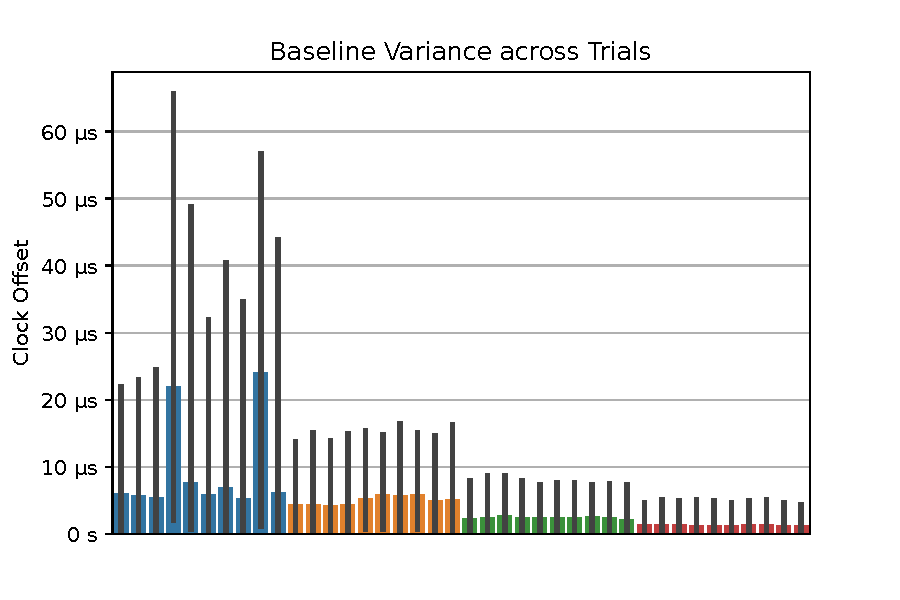
\includegraphics[width=\linewidth]{res/generated/base/key_metric_variance_rpi-4.pdf}
    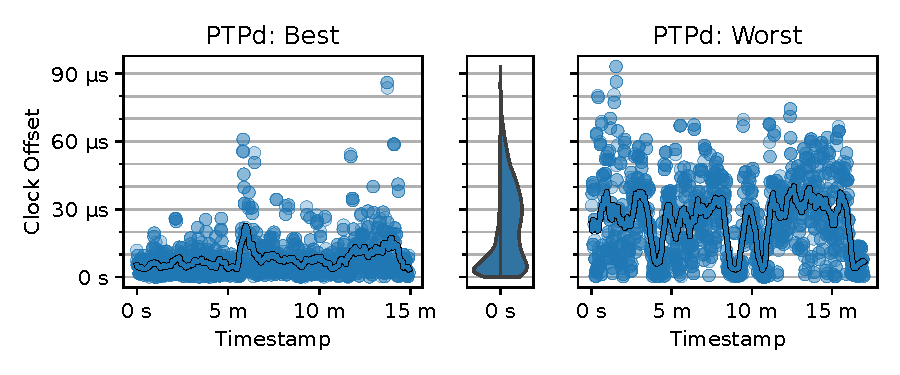
\includegraphics[width=\linewidth]{res/generated/base/ptpd-good-vs-bad.pdf}

    \legend
    \caption{Validating the baseline results by repeatedly measuring the baseline for both vendors on the Raspberry Pi 4 system. Top: The median absolute clock offset for each run, with error bars reaching from \PFive{} to \PNineFive{}. Bottom: Timeseries profiles for the best run and the worst run of PTPd under identical conditions, showing significant differences in noise levels.}
    \label{fig:baseline_reproducibility}
\end{figure}


{
\pgfkeys{
    /reproducibility/rpi-4/.cd,
    ptpd/min/.initial={0.000005329},
    ptpd/median/.initial={0.000005976},
    ptpd/max/.initial={0.000024082},
    linuxptp/min/.initial={0.0000041995},
    linuxptp/median/.initial={0.0000049845},
    linuxptp/max/.initial={0.0000059645},
    sptp/min/.initial={0.000002234},
    sptp/median/.initial={0.000002448},
    sptp/max/.initial={0.0000027660000000000003},
    chrony/min/.initial={0.00000125},
    chrony/median/.initial={0.0000012990000000000002},
    chrony/max/.initial={0.0000014060000000000002},
}
\renewcommand{\ptpKeyPrefix}{/reproducibility/rpi-4}



\newcommand{\numBaselineMeasurements}{10}
\newcommand{\baselineTotalMinutesRuntime}{\numBaselineMeasurements*4*2*20}
\newcommand{\numSamplesPerRunApprox}{\fpeval{round(20*60)}}

A key challenge with conducting quality performance studies aggregating data to increase information density while avoiding hiding important trends and outliers. While comparing clock-synchronization quantiles between vendors is certainly useful, in reality this does not tell the entire story because each baseline consists of a number of independent measurements, which in turn consists of around \numSamplesPerRunApprox{} samples, all of which are affected by multiple sources of noise. As it turns out (Figure~\ref{fig:baseline_reproducibility}), not only is there a significant amount of noise during each run\todo{Find a good metric to use here, perhaps std-dev + chebyshev law to deduce some intervals}, but there are also discrepancies between measurement runs. This leads to completely different results for identical measurement runs despite decent measurement lengths and number of samples.
\cmpSearchVendor{\ptpKey{\vendor/max}/\ptpKey{\vendor/min}}

\assert{\cmpMaxArg}{ptpd}
We observe that in absolute terms, PTPd is the main source of variance for both median/\PNineFive{} observed clock offsets and path delays across independent measurements. A simple restart of the PTPd client can suddenly cause the median latency to jump from \fTimeKey{ptpd/min} up to \fTimeKey{ptpd/max}, which corresponds to an increase of \fRelative[-1]{\ptpKey{ptpd/max}/\ptpKey{ptpd/min}} not only momentarily, but throughout an entire run of 20 minutes.
%This already comes uncomfortably close to our safety factor of \safetyMargin, and we have not even started stressing the system yet.
Fortunately, LinuxPTP produces a lot more stable results, with a smaller range of \fTimeKey{linuxptp/min} and \fTimeKey{linuxptp/max} between the best observed run and the worst observed run, corresponding to just \fRelative{\ptpKey{linuxptp/max}/\ptpKey{linuxptp/min}} difference. The best vendor in this regard is \fVendor{\cmpMinArg}, with both a relative range of just \fRelative{\cmpMin} and an absolute range of \fTime[1]{\ptpKey{chrony/max}-\ptpKey{chrony/min}}.
%
% Assert last sentence
\assert{\cmpMaxArg}{ptpd}
%

To deal with the amount of noise, we apply a variety of noise reduction techniques. All measurements are interleaved for better compensation of noise that may be introduced through mechanisms outside our control, we repeat each observation at least \numBaselineMeasurements{} times for each vendor on each hardware platform (totaling in around \fpeval{round(\baselineTotalMinutesRuntime/60)} hours of runtime and \fpeval{round(\baselineTotalMinutesRuntime*60)} samples collected for just one type of benchmark) and between each measurement run, the entire cluster is restarted to ensure that no state is carried over, which would harm the independence of observations. Otherwise, the setup is left undisturbed as far as possible, so that the only differences occur in the internal state of PTP. We further filter data that contains too many holes, undercuts a threshold of the actual number of samples collected, or fails basic consistency checks (all of which lead to bad quality data). The remaining data for the baseline is quite complete -- missing samples account for less than 0.1\% of data for each vendor and board.

The baseline, however, only shows observations under close to ideal circumstances. Despite that, we already observe some amount of synchronization quality variability.
Needless to say, a vendor that cannot deliver stable timing guarantees is risky to deploy in a production environment that needs to rely upon the time source functioning. In the upcoming sections, we will examine whether PTP clients can be made resilient against potential external and internal influences.

}

\section{Resource Contention}
\label{sec:resource_contention}

One aspect that influences how reliable PTP can operate is interference originating from resource sharing. Through our research, we examined a range of shared resources that might impact synchronization accuracy and thus need to be carefully managed so that PTP can provide synchronization even in the presence of stress. Unsurprisingly, the key resource tends to be network traffic.

\subsection{Network Contention}
\cmpSearchVendor{\ptpKey{load/net_unprioritized/load_100/rpi-4/\vendor/q95}/\ptpKey{base/rpi-4/\vendor/q95}}
\cmpSave{load/net_unprioritized/q95}
\cmpSearchVendor{\ptpKey{load/net_unprioritized/load_100/rpi-4/\vendor/q50}/\ptpKey{base/rpi-4/\vendor/q50}}
\cmpSave{load/net_unprioritized/q50}

\begin{figure}
    \centering
    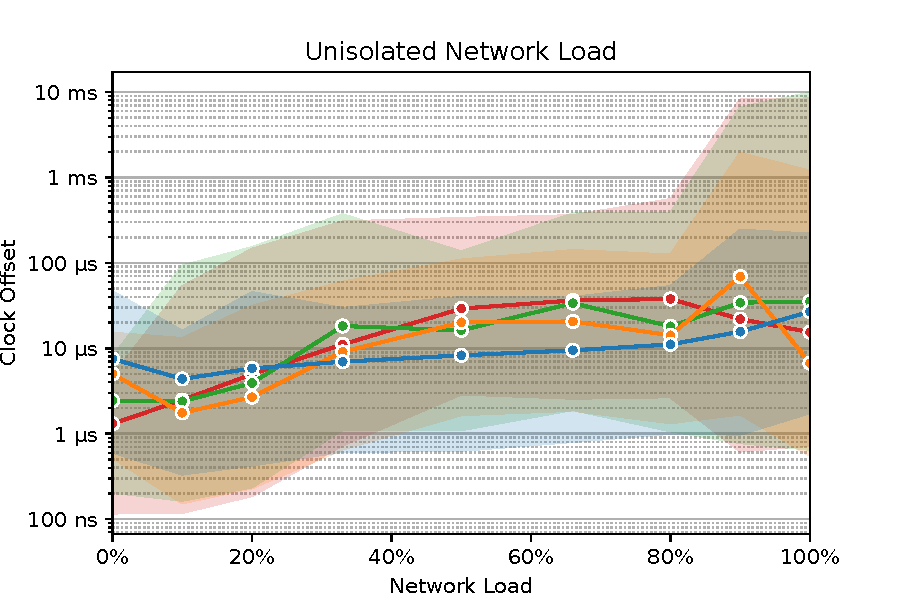
\includegraphics[width=\linewidth]{res/generated/net_unprioritized_trend_rpi-4.pdf}
    \legend
    \caption{Clock synchronization accuracy at different levels of network load. All vendors experience degradation at higher network loads, though the degree to which they are affected differs (\cmpLoad{load/net_unprioritized/q50}\fRatio{\cmpMin}--\fRatio{\cmpMax}). Apart from a change in median clock offset, \PNineFive{} is heavily affected, signaling larger and more frequent outliers of magnitudes \cmpLoad{load/net_unprioritized/q95}\fRatio[-1]{\cmpMax} as large as the baseline.}
    \label{fig:network_load}
\end{figure}


\cmpLoad{load/net_unprioritized/q50}
Like stated previously, the synchronization accuracy principally depends on the magnitude and the variation of the path delay. Intuition therefore suggests that the more network load is present, the more PTP will struggle to measure the clock offset consistently due to increased queuing in software and hardware causing delay and delay variation in delivery. We simulate network load artificially using iPerf, a traffic generator that allows us to target predefined data rates. By default, there are no special precautions in place to guard against network traffic contention out of the box, so a decrease in accuracy as the network load increases is exactly what we observe (Figure \ref{fig:network_load}\todo{Add vertical lines so its easier to judge}\todo{Data looks less neat again}). Interestingly, the vendor with the smallest increase in clock offset is \fVendor{\cmpMinArg}, with an increase of just \fRatio[1]{\cmpMin} (\fTimeKey{base/rpi-4/\cmpMinArg/q50} -- \fTimeKey{load/net_unprioritized/load_100/rpi-4/\cmpMinArg/q50}) from no network load to 100\% network load. On the other hand, \fVendor{\cmpMaxArg} has a much higher ratio of \fRatio{\cmpMax} (\fTimeKey{base/rpi-4/\cmpMaxArg/q50} -- \fTimeKey{load/net_unprioritized/load_100/rpi-4/\cmpMaxArg/q50}), which can only be partially attributed to the fact that \fVendor{\cmpMaxArg} has a smaller baseline value.
% Assert SPTP is worst
\assert{\cmpMaxArg}{sptp}%
SPTP is the only vendor that relies solely on unicast message exchange (a design choice by Meta), whether this is why SPTP appears to be more susceptible to contention is subject to further investigation.%
%
% 95-th percentiles
\cmpSearchVendor{\ptpKey{load/net_unprioritized/load_100/rpi-4/\vendor/q95}/\ptpKey{base/rpi-4/\vendor/q95}}%
\cmpSave{net_load_vs_baseline} % Used in conclusion
\PNineFive{} reflects the behavior of the outliers, and here we can observe even larger ranges, with \fVendor{\cmpMaxArg} now showing a ratio of \fRatio[-1]{\cmpMax} (\fTimeKey{base/rpi-4/\cmpMaxArg/q95} -- \fTimeKey[-1]{load/net_unprioritized/load_100/rpi-4/\cmpMaxArg/q95}). This is clearly above and beyond even very generous safety margins, so we need to examine how the effect of network load can be mitigated.

\begin{figure}
    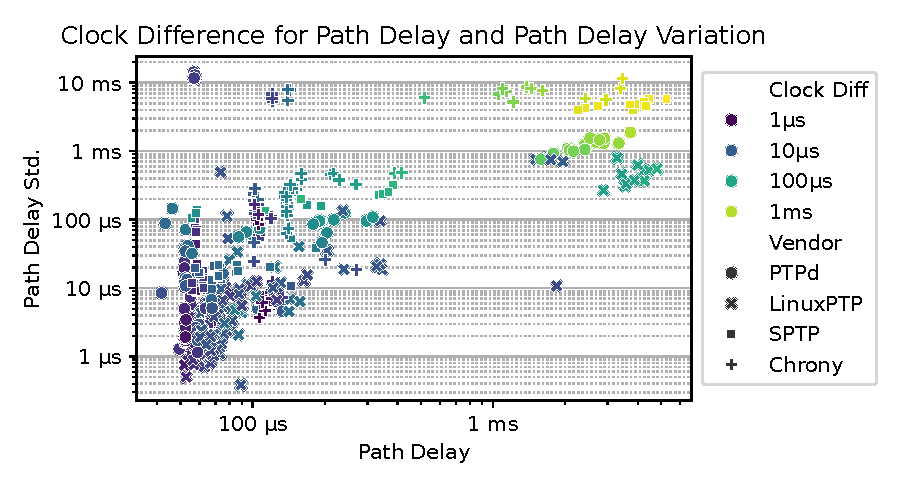
\includegraphics[width=\linewidth]{res/generated/base/clock_diff_by_path_delay.pdf}
    \caption{Resulting clock differences depending on the magnitude of the path delay and its variance, for all PTP implementations across all systems and under various tested circumstances. Each example represents a 20-minute measurement run.}
    \label{fig:path-delay-all}
\end{figure}

To show that the path delay is a good predictor of the synchronization quality, we can aggregate all 20-minute profiles across all our measurements and plot them by path delay and path delay variation (Figure~\ref{fig:path-delay-all}\todo{Make caption more clear}, \todo{Color scheme, color bar}). This shows us that generally, a high path delay and path delay variation is strongly correlated with a bad synchronization quality. However, each metric alone is not a good indicator as examples of high-quality synchronization are present wither either only high path delay or only high path delay variation. Notice also that there are multiple isolated clusters very far away from the norm (sometimes more than 10$\times$), which, while small, still have multiple examples often originating from the same vendor. This suggests that the internal path delay compensation mechanisms of these vendors can be tripped off balance more or less consistently.

\newcommand{\loadFaultyNumFailures}{9}
\newcommand{\loadFaultyNumTrials}{34}
Note that under heavier network load, PTP sometimes fails to even synchronize at all, when it gets stuck in an infinite loop of transmission timeouts indefinitely cycling between ``state init'' and ``state faulty''. In this case the timing system breaks entirely, and no synchronization can be established. These measurements have been excluded from the shown data, but we encountered them rather frequently at high load levels ($\sim$\fPercentage{\loadFaultyNumFailures/\loadFaultyNumTrials} of 20 minute runs for 100\% network load on the Raspberry-Pi 5 did not synchronize at all, with LinuxPTP accounting for most failures while Chrony produced no errors). Preventing this is paramount, as having no synchronization and potentially not even being aware of it is a lot worse than having a bad quality signal.

\begin{figure}
    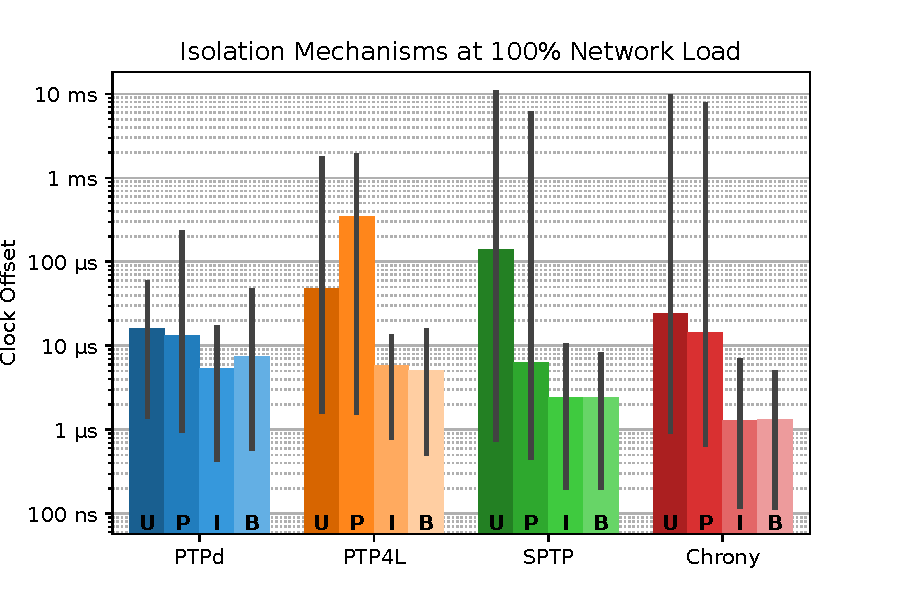
\includegraphics[width=\linewidth]{res/generated/net_isolation_comparison.pdf}
    \begin{center}
    \vspace{-0.5cm}
    \sffamily\scriptsize \textbf{U}: Unprioritized \quad\textbf{P}: Prioritized \quad\textbf{I}: Isolated \quad\textbf{B}: Baseline
    \end{center}
    \begin{center}
    \legend
    \end{center}
    \caption{Different possibilities of isolating the network load, compared to the baseline with no load. Both prioritization and physical isolation can often improve performance over the unprioritized default, however only isolation can match the performance of the baseline without resource contention.}
    \label{fig:net_isolation_comparison}
\end{figure}

Depending on the possibility of dedicating exclusive resources to PTP, two principle solutions are viable: a software/hardware prioritization of traffic to reduce interference of lower priority traffic and providing a dedicated network interface for physical isolation. While the latter might seem like an expensive proposition and could therefore be less suited for embedded solutions, other use cases like industrial or datacenter settings will often already provide a second management interface separate from the application's network. On our Raspberry-Pis, we emulate this by configuring the routing table so only PTP traffic can use the wired interface, with other traffic being relegated to the wireless interface. Figure~\ref{fig:net_isolation_comparison} shows these possibilities, with the default unisolated case on the left and the baseline on the very right.%
\cmpSearchVendor{\ptpKey{load/net_isolated/load_100/rpi-4/\vendor/q50}/\ptpKey{base/rpi-4/\vendor/q50}}%
%Worst: \fRatio[1]{\cmpMax} @ \cmpMaxArg{} and \fRatio[1]{\cmpMin} @ \cmpMinArg
\assertRange{\cmpMax}{1.0}{1.5}%
\assertRange{\cmpMin}{0.6}{1.0}%
Conforming to expectations, a physical isolation of PTP traffic can entirely mitigate the adverse effects of network load, with results sometimes even outperforming the baseline slightly (\fVendor{\cmpMinArg}: \fRelative{\cmpMin}, \fVendor{\cmpMaxArg}: \fRelative{\cmpMax}).
Theoretically, the only interference that could traverse the isolation barrier is latency caused by cross-talk on the software network stack, which does not appear to be an issue here.

The prioritization-based solution, however, cannot quite achieve the same level of performance on our testbed. Prioritization is achieved through differentiated services (via the Differentiated Services Code Point, DSCP), and requires prioritization support on every networking software and hardware component on the critical path to perform optimally. While our switch and operating system claim to support the technology, this does not appear to be sufficient for complete traffic segregation.
\cmpSearchVendor{\ptpKey{load/net_unprioritized/load_100/rpi-4/\vendor/q50}/\ptpKey{load/net_prioritized/load_100/rpi-4/\vendor/q50}}
Compared to no traffic prioritization, activating DSCP results in performance improvements up to \fRatio{\cmpMax} for \fVendor{\cmpMaxArg}.
However, one anomaly exists, which is \fVendor{\cmpMinArg}, where the median vendor performance actually decreases by \fRatio{1/\cmpMin}, while \PFive{} and \PNineFive{} remain within 3$\times$ the baseline.
\assertRange{\cmpMin}{0.01}{0.1}%
\assertRange{\ptpKey{load/net_unprioritized/load_100/rpi-4/linuxptp/q95}/\ptpKey{load/net_prioritized/load_100/rpi-4/linuxptp/q95}}{0.3}{1.0}%
\assertRange{\ptpKey{load/net_unprioritized/load_100/rpi-4/linuxptp/q5}/\ptpKey{load/net_prioritized/load_100/rpi-4/linuxptp/q5}}{0.3}{1.0}%
%
\newcommand{\numTrials}{min(\ptpKey{load/net_unprioritized/load_100/rpi-4/linuxptp/count}, \ptpKey{load/net_prioritized/load_100/rpi-4/linuxptp/count})}%
We have examined the affected profiles in more detail and can confirm that this effect is visible on all \fNum{\numTrials} trials encompassing approximately \fNum{\numTrials * 20 * 60} samples, so while we are confident of the validity of the observation, the reason why it occurs is currently unknown.

\todo{Perhaps recommendations}

\subsection{Other shared resources}

\cmpSearchVendor{\ptpKey{load/cpu_unprioritized/load_100/rpi-4/\vendor/q50}/\ptpKey{base/rpi-4/\vendor/q50}}
\cmpSave{q50}
\cmpSearchVendor{\ptpKey{load/cpu_unprioritized/load_100/rpi-4/\vendor/q95}/\ptpKey{base/rpi-4/\vendor/q95}}
\cmpSave{q95}

We have  further examined the effect of contention on other shared resources, and fortunately none of them cause synchronization quality degradation at the level that network congestion does.
An educated guess for the next most important shared resource could be CPU, as difficulties to get scheduled timely intuitively could cause delays in packet processing.
However, our data shows this is not the case on the Raspberry-Pi 4, as CPU contention only causes a maximum observed median degradation of just \cmpLoad{q50}\fRelative{\cmpMax} (\fVendor{\cmpMaxArg}) and \cmpLoad{q95}\fRelative{\cmpMax} at \PNineFive{} on the Raspberry-Pi 4, which is small enough not to make a practical difference.
\assert{\cmpMaxArg}{chrony}
This is likely due to the fact that PTP clients do not consume much processing time, which means they can easily get scheduled on Linux's Completely Fair Scheduler (CFS) even when idle computing time is scarce.
Interestingly, CPU load can actually boost performance relative to the baseline for \cmpLoad{q50}\fVendor{\cmpMinArg} by around \fRelativeInverted{\cmpMin} for the median value and \cmpLoad{q95}\fRelativeInverted{\cmpMin} for \PNineFive{} (\ptpKey{load/cpu_unprioritized/load_100/rpi-4/\cmpMinArg/count} trials, $\sim$\fNum{\ptpKey{load/cpu_unprioritized/load_100/rpi-4/\cmpMinArg/count} * 20 * 60} samples).
\cmpLoad{q50}\assertRange{\cmpMin}{0}{0.8}% Anything below 1 is decrease
\cmpLoad{q95}\assertRange{\cmpMin}{0}{0.8}% Anything below 1 is decrease
\assert{\ptpKey{cmp/q50/minarg}}{\ptpKey{cmp/q95/minarg}}%
%
We assume that this benefit originates from less scheduling variance when the processor is kept busy due to less power saving.
\cmpSearch{\vendor}{chrony,linuxptp,sptp}{\ptpKey{load/cpu_unprioritized/load_100/rpi-5/\vendor/q50}/\ptpKey{base/rpi-5/\vendor/q50}}%
\assertRange{\cmpMax}{1.0}{1.2}%
On the Raspberry-Pi 5, things look a little different. While Chrony, LinuxPTP and SPTP are mostly unaffected (up to just \fRelative{\cmpMax} overhead),
\cmpSearch{\vendor}{ptpd}{\ptpKey{load/cpu_unprioritized/load_100/rpi-5/\vendor/q50}/\ptpKey{base/rpi-5/\vendor/q50}}%
\assertRange{\cmpMin}{1.6}{3.0}%
PTPd has a more noticeable degradation in synchronization performance of up to \fRelative{\cmpMax}, which is however not nearly as critical as the previous degradation through network congestion.

\cmpSearchVendorCluster{\cmpRatioVendorClusterVsBaseline{load/aux_cache/load_100}}%

\assertRange{\cmpMin}{0.8}{1.2}
\assertRange{\cmpMax}{8.0}{10.0}
\cmpSave{cache}%
The third principal hardware component where contention can occur is the memory hierarchy. Generally, PTP does not require a large amount of memory to function, but we do observe a moderate amount of sensitivity both against cache contention on some systems (up to \fRatio[1]{\cmpMax} with \fVendorCluster{\cmpMaxArg}) while others are relatively unaffected (\fRatio[0]{\cmpMin} with \fVendorCluster{\cmpMinArg}),%
\cmpSearchVendorCluster{\cmpRatioVendorClusterVsBaseline{load/aux_memory/load_100}}%
%\assertRange{\cmpMin}{0.8}{1.2}%
%\todo{TODO: RE-ENABLE ASSERTION WHEN DATA AVAILABLE}
\assertRange{\cmpMax}{8.0}{10.0}%
\cmpSave{memory}%
and memory bandwidth contention (between \fRatio[0]{\cmpMin} with \fVendorCluster{\cmpMinArg} and \fRatio{\cmpMax} with \fVendorCluster{\cmpMaxArg}).
\assertRange{\cmpKey{memory}{max}}{\cmpKey{cache}{max}*0.8}{\cmpKey{cache}{max}*1.2}%
In the end, both memory bandwidth contention and cache contention turn out to be more important than CPU contention.%
% q50 is cpu_unprioritized, ugh.
\assertRange{\cmpKey{q50}{max}}{0}{\cmpKey{memory}{max}*0.75}%

% For conclusion
\cmpSearchVendorCluster{max(\cmpRatioVendorClusterVsBaselineQNineFive{load/aux_memory/load_100}, \cmpRatioVendorClusterVsBaselineQNineFive{load/aux_memory/load_100})}%
\cmpSave{cache_mem_vs_baseline}

We have put the PTP clients through further stress tests (leveraging the capabilities provided by Stress-NG) and observe the following:%
\begin{itemize}
    \item Stressing time-related kernel features such as timers or alarms do not impact PTP performance significantly (with a maximum deviation from the baseline of under 50\%).
    \cmpSearchVendorCluster{\cmpRatioVendorClusterVsBaseline{load/aux_timer/load_100}}%
    \assertRange{\cmpMax}{0.5}{1.5}%
    \cmpSearchVendorCluster{\cmpRatioVendorClusterVsBaseline{load/aux_alarm/load_100}}%
    \assertRange{\cmpMax}{0.5}{1.5}%
    \item Installing cyclic tasks with a deadline in the schedule (\texttt{SCHED\_DEADLINE}), which might cause PTP to get deferred when a real-time task needs to be scheduled, also do not cause significant adverse effects. This is good news as applications that require precise notions of time will often also be time-critical, and thus they usually use a real-time scheduling policy. However, note that things will likely start to fall apart when real-time tasks hog almost all available compute, as this will make it difficult for PTP to get scheduled at all unless it is promoted to a corresponding scheduling policy itself (which is not the case for the default profile).
    \cmpSearchVendorCluster{\cmpRatioVendorClusterVsBaseline{load/aux_cyclic/load_100}}%
    \assertRange{\cmpMax}{0.5}{1.5}%
    \item Finally, all PTP implementations also show good resilience against excessive context switching, which places stress on multiple software and hardware components simultaneously.
    \cmpSearchVendorCluster{\cmpRatioVendorClusterVsBaseline{load/aux_switch/load_100}}%
    \assertRange{\cmpMax}{0.5}{1.5}%
\end{itemize}

While resource contention, especially network congestion, can lead to degradation of clock synchronization performance, it is not the sole reason that the time synchronization system may fail.

%Interestingly, some level of load can actually boost performance relative to the baseline (we observed this on both the CPU and the network).
%We assume this occurs due to the hardware switching less into power saving states when more load is present, which may actually cause packets to be delivered faster.

\section{Fault Tolerance}
\label{sec:fault_tolerance}
\newcommand{\faultLength}{30 seconds}
%\todo{Review this: The information density of this section needs to be increased}

\begin{figure}
    \begin{center}
    \begin{tikzpicture}[component/.style={draw}, node distance=0.5cm]
        \node[component, ] (master) {\faBug{} \faBolt{} Master};
        \node[component, right=of master] (network) {\faBolt{} Network};
        \node[component, right=of network] (primary-slave) {\faBug{} \faBolt{} Primary Slave};
        \node[component, below=0.25cm of primary-slave] (secondary-slave) {Secondary Slave*};

        \draw[-] (master) -- (network);
        \draw[-] (network) -- (primary-slave);
        \draw[-] (network) |- (secondary-slave);
    \end{tikzpicture}
    \end{center}

    \scriptsize *: For certain outlined scenarios, the secondary slave gets promoted to a failover master when the master fails.

    \caption{
        Simple fault-setup consisting of three clients, where potential software (\faBug{}) or hardware (\faBolt{}) faults may occur. Since we exclude compound failures, only one fault can occur simultaneously, so no faults are triggered in the secondary slave.
    }
    \label{fig:fault_architecture}
\end{figure}

Apart from resource contention, faults are another key threat to the functioning of the timing system. We examine faults originating from three distinct causes: a fault in the PTP software, a fault in a node's hardware, and a fault on the network. The software/hardware faults can either occur on a PTP slave (less critical as failures are expected to be contained within a node), or on the PTP master, in which case they are more critical as the failure could propagate across the PTP domain. In high-reliability deployments, there will typically be a failover master to take over upon a fault in the master, so we examine that scenario too. Figure~\ref{fig:fault_architecture} shows an overview of the locations and types of faults that may occur.

\subsection{Software Fault -- Slave}

\cmpSearchVendor{\ptpKey{fault/software/slave/rpi-4/\vendor/count}}
\xdef\bSoftwareFaultNumProfiles{\cmpMax}
\newcommand{\maxClockSlew}{(0.05/100)}
\newcommand{\windowOfUncertaintyOneMinute}{(60*(\maxClockSlew))}

\begin{figure}
    \centering
    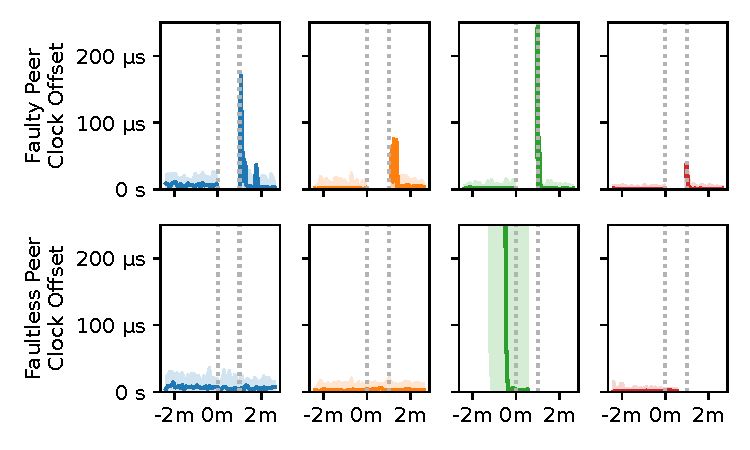
\includegraphics[width=\linewidth]{res/generated/fault/software/slave_rpi-4_peer_comparison.pdf}
    \legend
    \caption{Faults induced by a software crash on Raspberry-Pi 4, with a faulty client (top) and a second client as a control (bottom). Just after the fault, an increased offset can be observed as PTP tries to resynchronize the clock. Since these offsets occur randomly, we superimpose \fNum{\bSoftwareFaultNumProfiles} trials for each vendor so that the worst case can be seen.}
    \label{fig:software_fault}
\end{figure}

The simplest possible fault is a PTP client crashing, because the only state that is lost is within the PTP slave client application (such as the state of the servo disciplining the clock). We emulate software faults via SIGKILL, forcefully terminating the PTP client -- in reality such a fault might come from within the client due to e.g. a bug, or from an external source (e.g. a process kill during an out-of-memory situation). While the PTP application is down, the clock will continue to drift at the real clock drift rate minus the compensation rate that was last set by the PTP application. If the synchronization before the crash was stable, this observed drift rate is expected to be comparatively low. However, in the worst case when the clock slew is at the maximum rate (as will often be the case in the early stages of convergence), the software-driven drift can be up to 0.05\%~\cite{adjtimex}, which can cause a software-induced drift of \fTime{0.05/100} per second of downtime, or \fTimeMS{\windowOfUncertaintyOneMinute} per minute. We wish to determine empirically how big the offset is from a software fault when the clock is stable.

\cmpSearchVendor{\ptpKey{fault/software/slave/rpi-4/\vendor/fault/post_max/min}}
\cmpSave{fault/software/post_max/min}
\cmpSearchVendor{\ptpKey{fault/software/slave/rpi-4/\vendor/fault/post_max/max}}

From the results (Figure~\ref{fig:software_fault} top), we can determine that the maximum observed offset after a 1-minute software fault among \fNum{\bSoftwareFaultNumProfiles} trials is \fTime{\cmpMax} for \fVendor{\cmpMaxArg}, which is around \fRatio{\cmpMax/\ptpKey{base/rpi-4/\cmpMaxArg/q50}} worse than the median baseline performance. Fortunately, this drift is far from the theoretical worst-case window of uncertainty of \fTimeMS{\windowOfUncertaintyOneMinute}, representing just \fPercentage[1]{\cmpMax/\windowOfUncertaintyOneMinute} of the maximum software induced drift. We also observe that it is possible to get lucky: in some trials there is very little observed offset despite a full minute of downtime ({just \cmpLoad{fault/software/post_max/min}\fTime{\cmpMin} with \fVendor{\cmpMinArg}}'s best trial). In any case, all PTP implementations can quickly reconverge on the clock signal within a few seconds of restarting. Due to a quirk in how the PTP protocol works (slaves request synchronization signal leases from the master with a predetermined expiry), the master node will keep sending synchronization messages to the dead peer (abandoned sync~\cite{sptp}), which combined with the second lease that is issued when the PTP slave is restarted can help the peer synchronize even quicker due to the higher influx of synchronization messages.

\cmpSearch{\vendor}{ptpd,linuxptp}{\ptpKey{fault/software/slave/rpi-4/\vendor/fault/secondary/post_max/max}}

In high-reliability deployments, it is important to ensure that faults stay contained and cannot propagate. In terms of PTP, this means that slave-side faults should not affect the synchronization quality of other slaves. To verify that this is the case, we attached a second control node to the same master (Figure~\ref{fig:software_fault} bottom\todo{Add graphic title}), which shows us some mixed behavior: There is no meaningful degradation of the performance of the secondary slave for PTPd and LinuxPTP (maximum value after fault \fTime[0]{\cmpMax} for \fVendor{\cmpMaxArg} is smaller than the baseline), but SPTP and Chrony show difficult to explain behavior: among all trials, we observe temporary disconnects between 7\,min--2\,min before the fault and from 1\,min after the fault to the end of the profile at 4\,min for SPTP (showing error: failed to get timestamp of last packet: no TX timestamp found after 10 tries (500 ms)). This is especially notable because Chrony shows exactly the same outages at the same times (error: can't synchronise: no selectable sources), consistently reproducible to second accuracy (the visual difference results because SPTP converges slowly and thus most of the trajectory is out of view).
\assertRange{\cmpMax}{0.000010}{0.000035}

One important caveat is to be noted for PTPd: when multiple software faults start occurring (not necessarily in close proximity to each other), problems can start propagating. On our test systems, we observe that upon exactly the third software fault, PTPd will cause the network interface to fail. In fact, no amount of manually bringing the network down and back up or reloading the network interface driver can solve this problem, up until the system is restarted by hand. This is especially critical as it implies that not only will the timing system fail, but it will simultaneously bring down any applications that need to communicate over the interface as well. Ironically, in this case, rather than support the deployment of high-reliability distributed systems, PTPd will actually harm said reliability. We thus advise caution when deploying PTPd or any of its derivatives that may contain the same bug.

\subsection{Hardware Fault -- Slave}
\cmpSearchVendor{\ptpKey{fault/hardware/slave/rpi-4/\vendor/fault/post_max/max}}
\xdef\maxPiFour{\cmpMax}
\cmpSave{hw_slave_rpi-4}

\cmpSearchVendor{\ptpKey{fault/hardware/slave/rpi-5/\vendor/fault/post_max/max}}
\xdef\maxPiFive{\cmpMax}
\cmpSave{hw_slave_rpi-5}


\begin{figure}
    \centering
    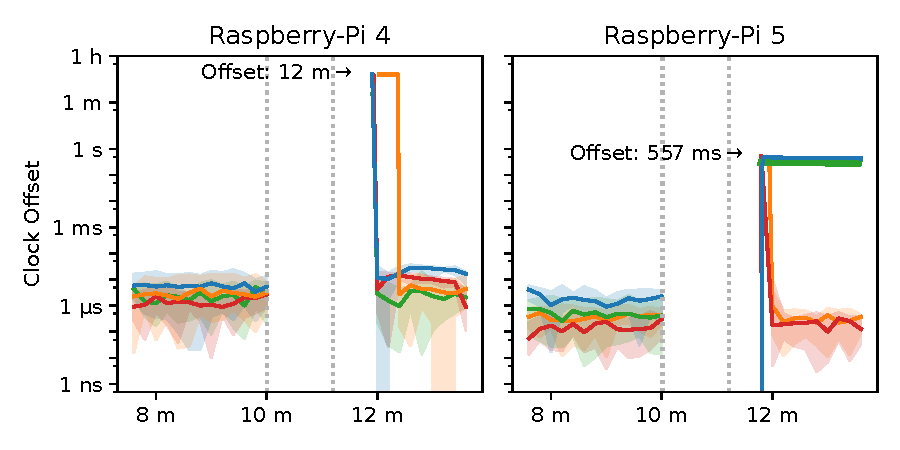
\includegraphics[width=\linewidth]{res/generated/fault/hardware/slave_cluster_comparison.pdf}
    \legend
    \caption{A hardware fault on the slave of the Raspberry-Pi 4 cluster (left) and the Raspberry-Pi 5 cluster (right). Both slaves need to fully resynchronize after rebooting, but the Raspberry-Pi 5 has an advantage due to its hardware clock. However, if the offset is just under 1 second then lengthy reconvergence can occur. Unfortunately, Xilinx and TK-1 boards are excluded as they cannot reboot after a power failure without a physical button press.}
    \label{fig:hardware_fault_slave}
\end{figure}

\begin{figure}
    \centering
    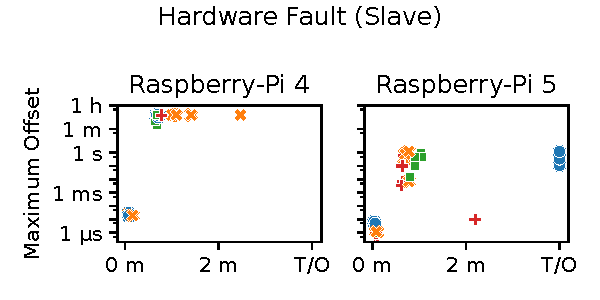
\includegraphics[width=0.7\linewidth]{res/generated/fault/hardware/slave/fault_scatter.pdf}
    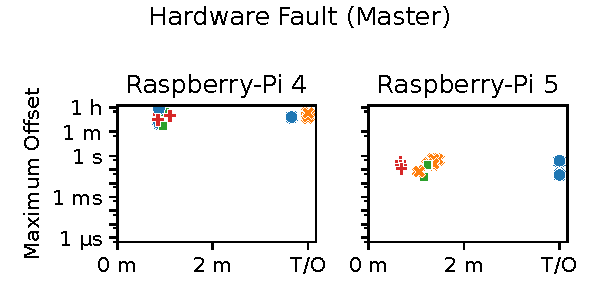
\includegraphics[width=0.7\linewidth]{res/generated/fault/hardware/master/fault_scatter.pdf}
%    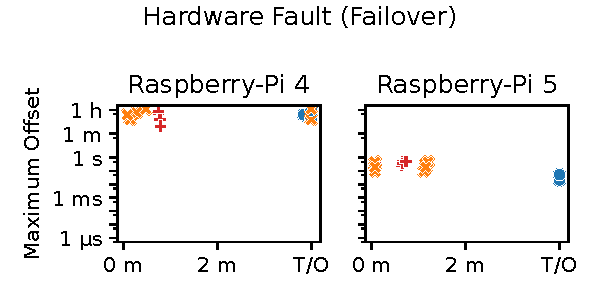
\includegraphics[width=0.7\linewidth]{res/generated/fault/hardware/master_failover/fault_scatter.pdf}
    \caption{The maximum clock offset observed and the time taken to reconverge to the normal accuracy (up to a 4 minute timeout) for different points of failure. Due to the missing real-time clock, the Raspberry Pi 4 observes high offsets sometimes indefinitely. The Raspberry Pi 5 has better resilience, but reconvergence can still take a long time.}
    \label{fig:fault_offsets}
\end{figure}

A slightly more difficult scenario is a hardware fault on the slave, as not only will the internal PTP state be lost, but also the kernel state containing the current system time and the clock drift. This implies that PTP will need to fully reconverge, using the standard step-and-slew approach seen in the baseline. We produce simulated hardware faults using our programmable power delivery unit, which is equivalent to a loss-of-power scenario, but real-life production hardware faults and system hang-ups could also come from other component failures. Because the Raspberry-Pi 4 (Figure~\ref{fig:hardware_fault_slave} left) does not contain a real-time clock to preserve the system time across reboots, after a reboot a node will have a system time equal the last time that the time was persisted to disk if fake-hwclock~\cite{fake-hwclock-manpage} is active or a default value (e.g. the epoch in 1970) if fake-hwclock is not active. On our system (Raspbian, which bases on Debian), fake-hwclock is configured, so we observe a temporary deviation of \cmpLoad{hw_slave_rpi-4}\fTimeMin{\cmpMax} (on \fVendor{\cmpMaxArg}). To fix the large offset, PTP steps the clock (breaking invariant I2) and then reconverges for some minutes on the previous level of accuracy (in the case of PTPd, we see the characteristic rebound).

On the other hand, the Raspberry-Pi 5 (Figure~\ref{fig:hardware_fault_slave} right) can maintain the current time using the hardware clock while it is not running. While the RTC generally has lower resolution than the internal oscillator (commonly 32768 Hz), it generally has good long-term stability\todo{cite}. This advantage shows itself in the observed maximum offset, which is a comparatively small \cmpLoad{hw_slave_rpi-5}\fTimeMS{\cmpMax} (\fVendor{\cmpMaxArg}), a full \fNum{ln(\maxPiFour/\maxPiFive)/ln(10)} orders of magnitude smaller, which can theoretically be compensated by clock slew only within the aforementioned \fTimeMin{1/(\maxClockSlew)}. This is what happens to PTPd: it skips the initial clock step in the default profile when the observed calibration offset is smaller than one second, opting for stability at the cost of a very long convergence time.

A fault on a system without a hardware clock will thus cause an application to encounter large inconsistencies in timing in a place where it might not expect it (right in the middle of a run), while a simple RTC can mitigate this problem entirely. For deployments that are stuck on systems where an RTC is not viable (e.g. due to cost reasons), it is recommended to configure a delay for the application relaunch to allow PTP to resynchronize first.

\subsection{Hardware Fault -- Master}

%\begin{figure}
%    \centering
%    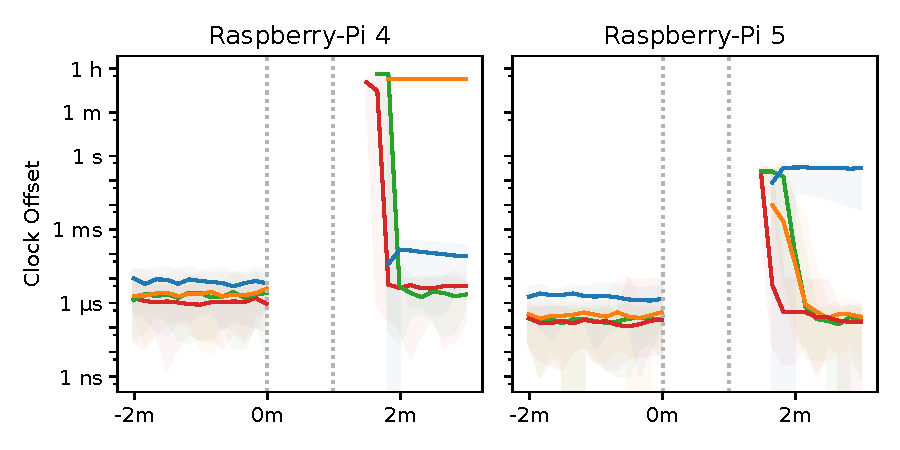
\includegraphics[width=\linewidth]{res/generated/fault/hardware/master_cluster_comparison.pdf}
%    \legend
%    \caption{A hardware fault on the master of the Raspberry-Pi 4 cluster (left) and the Raspberry-Pi 5 cluster (right). Slaves cannot compensate for unexpected changes in the announced time without correct configuration, so large clock offsets may be present practically indefinitely.}
%    \label{fig:hardware_fault_master}
%\end{figure}


PTP slaves are not the only type of node that can fail, the PTP master can just as well be affected by a disruption. Of all the scenarios, this is the most difficult one, as a failure will cause all slave nodes to become desynchronized. A failure on the master will inevitably also lead to inconsistencies in the announced time, especially in the embedded scenario where no external clock source for ground truth is available. On the Raspberry-Pi 4 (Figure~\ref{fig:fault_offsets} bottom), we observe that when the master restarts and now has a different reference time, there is once again a large offset between the master time and the times on the slaves akin to the earlier faults on the slaves (Figure~\ref{fig:fault_offsets} top). However, unlike previously, the slave nodes are not allowed to perform another clock step unless they have been configured to do so. The reason for this lies in the default configuration of the PTP clients: It is assumed that stable time needs to be served to the application, so invariants I1 and I2 may not be broken (except at initial startup). We observe however, that this behavior is not consistent for hardware faults on the master: sometimes the offset is compensated by clock step, sometimes slaves get stuck in a clock slew, which especially for the large observed offset of \fTimeMin{\maxPiFour} is projected to require at least \fTimeMin[-3]{\maxPiFour/\maxClockSlew} -- clearly impractical. Moreover, while the slaves are converging on the new master clock at close to the maximum slew rate simultaneously, we observe that they do not stay well in sync between each other while this happens, because the hardware clock drift continues to differ between nodes. This implies that remaining peers can also not rely on their clocks being close to each other either. This problem of indefinite clock-slew can be avoided by reconfiguring the PTP slave to also allow subsequent clock steps (which is disabled by default for safety), but the system should be well tested for resilience as the application will have to cope with a large magnitude rewinding of the clock (worst case: breaking both I1 and I2). Experimentation on the stress-test tools and other applications show that many applications misbehave during a clock step, so it cannot be assumed that an application is resilient simply because it uses Linux's monotonic clock.

As observed previously, the issue is somewhat mitigated by using an external clock that can maintain system time during downtime (e.g. Raspberry-Pi 5). The clock source does not need to be of particularly high quality if the goal is to only maintain sub-second synchronization accuracy, depending on the downtime. Should constraints only allow an external clock to be installed on a single node, intuition and our observations suggest that the primary target for installation should be the master node -- it can propagate its stable time source to the slaves.

\subsection{Hardware Fault -- Failover Master}

\begin{figure}
    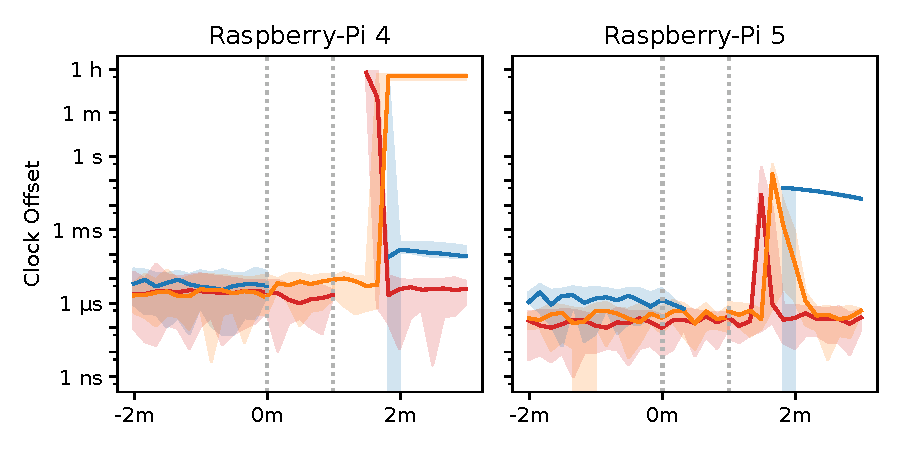
\includegraphics[width=\linewidth]{res/generated/fault/hardware/master_failover_cluster_comparison.pdf}
    \caption{Fault tolerance with a failover master. While the failover master works almost seamlessly (except for PTPd), problems arise when the original master eventually reboots and starts announcing the wrong time identically to the previous scenario without a failover.}
    \label{fig:failover}
\end{figure}

To increase service availability it is common to install a failover for any single point of failure in a distributed system so that the backup system can take over when the primary system fails. This is not only applicable for data-centers, but also applies to our minimal three node embedded setup, as a failover master will allow the two remaining nodes to remain synchronized with each other when the primary master fails. Fortunately, PTP was designed with this explicitly in mind so that the failover master does not necessarily require its own clock source, the failover node can automatically assume a slave state while the master is healthy (thus acquiring a clock signal consistent with the master's) and subsequently promote itself to a master when the original master is no longer healthy. Note that this setup is not supported in Meta's SPTP, as masters and slaves run different binaries and thus cannot switch roles dynamically (an external clock source would be necessary for two synchronized masters, we thus exclude SPTP from this evaluation).

\cmpSearchVendor{\ptpKey{fault/hardware/master_failover/rpi-4/\vendor/fault/post_max/max}}
\cmpSave{master_failover/rpi-4}
\cmpSearchVendor{\ptpKey{fault/hardware/master_failover/rpi-5/\vendor/fault/post_max/max}}
\cmpSave{master_failover/rpi-5}
We observe that the failover master can very rapidly take over the master role in the event of a failure for LinuxPTP and Chrony, causing virtually no disruption in the timing service\todo{Import numbers} (Figure~\ref{fig:failover}\todo{I don't like how Figure 14 looks, it seems confusing}). PTPd is not able to use the failover successfully (error: No active masters present, resetting port). However, even for LinuxPTP and Chrony the presence of a failover master cannot mitigate the problem of the master eventually restarting and disseminating the wrong time, which will be picked up by the failover master and the slaves, causing clock spikes and stepping of familiar magnitudes: \cmpLoad{master_failover/rpi-4}\fTimeMin{\cmpMax} on Raspberry-Pi 4 and \cmpLoad{master_failover/rpi-5}\fTimeMS{\cmpMax} on Raspberry-Pi 5. Due to the way the best master clock algorithm works (the same master clock will always be selected deterministically - unless the configuration is changed thus shifting the prioritization), the failover master cannot re-teach the current network time to the master that has just restarted because it does not take priority.
To mitigate this, three options are available: Either the master is permanently disabled upon a fault, it is reconfigured to a lower priority and thus becomes a slave, or it is ensured via an external clock source that a power fault does not cause a change in time.

\subsection{Network Fault}

\begin{figure}
    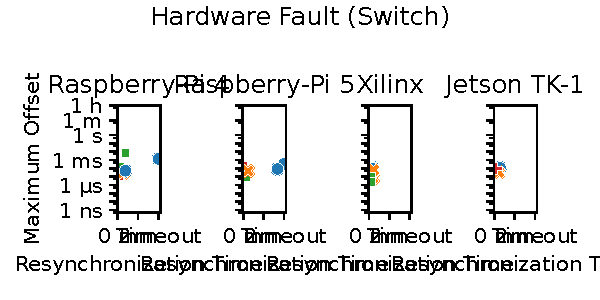
\includegraphics[width=\linewidth]{res/generated/fault/hardware/switch/fault_scatter.pdf}
    \caption{Network faults are the easy failure mode for timing systems, as most rely on connectionless socket types and no state is lost. PTPd also does not nearly require as much reconvergence time on Xilinx and Jetson Boards when compared to the Raspberry Pi.}
    \label{fig:network_fault}
\end{figure}

\cmpSearchVendorCluster{\ptpKey{fault/hardware/switch/\cluster/\vendor/fault/post_max/max}}
Another possible root cause for a fault is the network. While a network outage is generally bad news for reliable distributed systems that need to communicate, a total network outage is ironically easier for PTP to handle than a functioning network with high levels of congestion or a contained failure within any of the nodes. Since no state is lost, the servos are kept in holdover and PTP just has to detect when the network is available again to reconverge on the common network time (Figure~\ref{fig:network_fault}). Interestingly, PTPd, which has shown itself prone to indefinite clock-slew on Raspberry-Pi 4 and 5, does not suffer the same problem on Xilinx and Jetson TK-1. Generally, the post fault clock offsets are significantly better (worst: \fVendorCluster{\cmpMaxArg} with average \fTime[-1]{\cmpMax}) than any single node failing.

Overall, we observe that faults can break PTP systems in many perhaps unexpected ways, and that there is no bound on the magnitude of deviation that can occur. To get any degree of resilience out of a PTP network, careful configuration and testing is required. Vendors leave this mostly to the users by relying on profiles that the user needs to select/specialize to their requirements. Before distributed algorithms can effectively rely on network time sources on embedded systems, we need better predictability and ideally more consistent behavior across both boards and vendors.

\section{Resource Consumption}
\label{sec:resource_consumption}
%\todo{Find where to place this section.}

\begin{figure*}
\centering
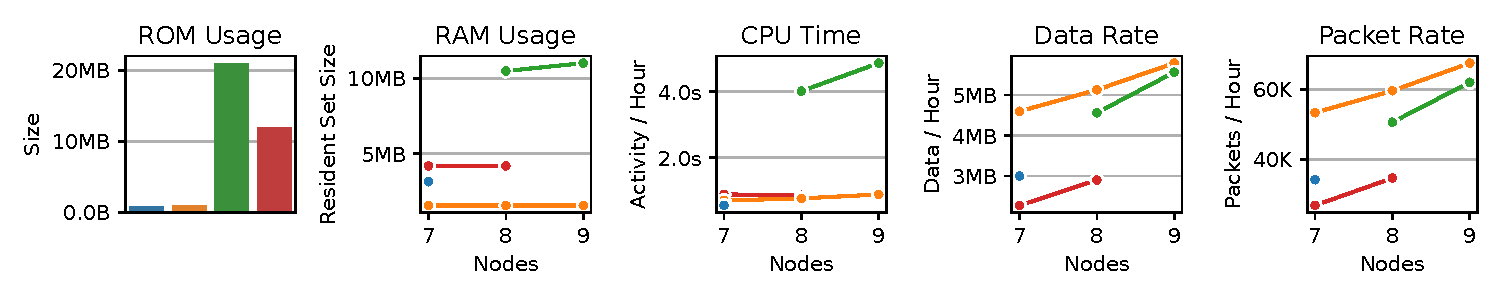
\includegraphics[width=\linewidth]{res/generated/resource_consumption/summary_trend.pdf}
\legend
\caption{Resource consumption statistics across vendors and systems. In general, PTP systems use few onboard resources but generate more network traffic, while the evaluated NTP and SPTP implementations reduce network utilization at the cost of additional ROM and other on-board resources. Note that SPTP only scales to 10 nodes as it cannot run on the final 2 TK-1 boards.}
\label{fig:resource_consumption}
\end{figure*}

\begin{figure}
\begin{center}
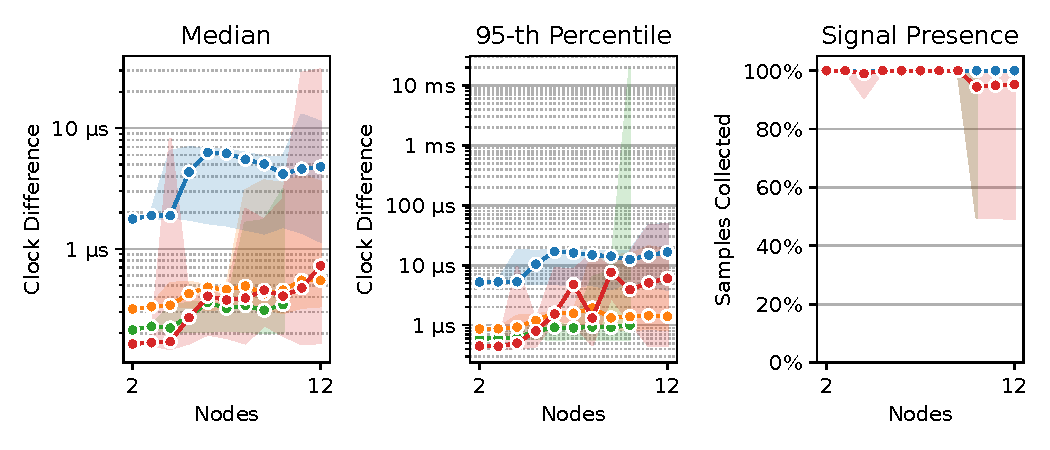
\includegraphics[width=\linewidth]{res/generated/resource_consumption/summary_quality_trend.pdf}
\legend
\end{center}

{\footnotesize {\bfseries Note:} The top end of the error band is the worst node's median/\PNineFive{}, the bottom end the best node's median/\PNineFive{}, respectively.}
\caption{Synchronization quality for increasing numbers of nodes, with clock difference median (left) and \PNineFive{} (center). As the number of nodes increases, some slaves start to occasionally lose the synchronization signal (right).}
\label{fig:resource_consumption_quality}
\end{figure}


Finally, embedded systems need to take particular care of the resource consumption of their applications. Since time synchronization fulfills only a supporting role in the overall deployment, it is important that it does not detract significantly from the resources available for the actual application. This is not only true for resources with a hard limit (compute, memory, etc.) but also for ``soft'' resources like power draw and heat dissipation. Especially SPTP was created with the intention of less resource consumption in mind~\cite{sptp}, so we will verify whether reality holds up to these claims.

While some PTP systems are specifically tied to Linux and thus come with the associated resource requirements, others can also be deployed in more lightweight environments. On low capability devices, ROM/flash space is generally restricted, so the footprint becomes a concern. To measure each implementation's ROM footprint, we strip packages of documentation and dependencies that can reasonably be expected to already be available (e.g. lib-c) but include other required dependencies in the calculation (Figure~\ref{fig:resource_consumption} left).
We find that PTPd requires the least ROM, with executables, data and dependencies totaling at around 840\,KB. The LinuxPTP package is larger but requires fewer dependencies, thus the resulting footprint of 970\,KB is around the same. SPTP (21\,MB) and Chrony (12\,MB) are both more than an order of magnitude larger due to the integrated Go runtime and the comparatively large number of dependencies, respectively. Note that the size of SPTP could be reduced by around 40\% by only deploying either the master or client executable and the Chrony footprint is significantly smaller if the larger dependencies (iproute2 + libgnutls30 + tzdata $=$ 10\,MB) are already available.
In combination with an embedded Linux distribution, the more lightweight systems could reasonably be deployed on 16\,MB flash devices, although this would likely not leave sufficient headroom for the actual application -- thus 32\,MB is the more realistic lower bound for PTP deployments.

Closely tied to the storage footprint is the memory footprint. LinuxPTP (250\,KB-400\,KB), Chrony (800\~KB-1\,MB) and PTPD ($\sim$1\,MB) all have reasonably small unique set sizes, with resident set sizes around 2-4\,MB. SPTP requires significantly more, with unique and resident set sizes starting at 8-10\,MB for the master node and 15-16\,MB on the slave. The memory consumption of SPTP is also growing much faster at \fNum[-1]{(12058624-9437184)/11/1000}\,KB for each additional slave (Figure \ref{fig:resource_consumption} center left) than the other vendors. Also notable is the virtual memory allocated by SPTP, 3\,GB on the master and 1\,GB on the client: over 100x more space than the next most hungry implementation (Chrony at 11\,MB) and enough to cause potential issues on 16-bit deployments and platforms that don't have large amounts of virtual memory available or that do not want to overcommit.

\cmpSearch{\i}{1,...,11}{\ptpKey{scalability/1_to_\i/big-bad/chrony/sys/proc/cpu}/min(\ptpKey{scalability/1_to_\i/big-bad/ptpd/sys/proc/cpu}, \ptpKey{scalability/1_to_\i/big-bad/linuxptp/sys/proc/cpu})}
\cmpSave{resource/cpu/chrony}

\cmpSearch{\i}{1,...,9}{\ptpKey{scalability/1_to_\i/big-bad/sptp/sys/proc/cpu}/min(\ptpKey{scalability/1_to_\i/big-bad/ptpd/sys/proc/cpu}, \ptpKey{scalability/1_to_\i/big-bad/linuxptp/sys/proc/cpu})}
\cmpSave{resource/cpu/sptp}


Aside from deployability, power consumption is another big concern especially for mobile deployments. Using consumed CPU time as a heuristic for power consumption, we observe that LinuxPTP and PTPd consume the fewest compute, while Chrony requires around \fRelative{\cmpKey{resource/cpu/chrony}{min}}$-$\fRelative{\cmpKey{resource/cpu/chrony}{max}}\% more. SPTP consumes the most cycles, starting at \fRelative[-1]{\cmpKey{resource/cpu/sptp}{min}} more consumption than LinuxPTP and PTPd and climbing up to \fRelative[-1]{\cmpKey{resource/cpu/sptp}{max}}, causing the master node to run \fNum[1]{52.7-51.3}°C hotter (indicative of the additional energy expended). Overall however, the consumption of compute power is reasonable even for SPTP, with the comparatively powerful ARM Cortex-A72 theoretically supporting around \fNum[-1]{1/0.002036022015381676} clients (linear extrapolation), more than enough for a typical embedded deployment.

Network traffic can also be a concern for low-throughput networks, but vendors claim that PTP uses a negligible amount of bandwidth~\cite{ptp-onestep-twostep-five-minute-facts}. Our results suggest that while the difference is less pronounced, SPTP still exceeds the other implementations with around 1.1\,MB and \fNum{31150*3/10/1000}K packets per hour and client. The exception to this is $n\leq2$, where SPTP matches or outperforms the PTP implementations. Chrony is most efficient with network resources, but with too small a margin to make any practical difference. PTPd and LinuxPTP are roughly equal on both data and packet rates, likely because they implement the same protocol.

Finally, resource efficiency is only a concern when clock synchronization is maintained. We evaluate synchronization quality by number of nodes in the domain (\cref{fig:resource_consumption_quality}), scaling from two nodes to the entire cluster in order of decreasing board capability (Master: R-PI 5, Slaves: 2$\times$R-Pi 5, 4$\times$Xilinx, 3$\times$R-Pi 4, 2$\times$TK-1). \todo{Describe once data more or less final.}

Overall, despite SPTP's promise of better resource efficiency~\cite{sptp} due simplifying the protocol, we cannot confirm this for our embedded testbed, but instead find it uses considerably more ROM, RAM, and compute (Figure~\ref{fig:resource_consumption}\todo{Figure resource consumption quality is not easy to interpret.}). Thus, it is actually less well suited to embedded deployments than the more widespread PTP vendors. However, this does not necessarily contradict the claims made in the SPTP article~\cite{sptp}, since the article targeted mass-scale deployments of 100K clients, a scale that is highly uncommon in the embedded world. For minimizing resource consumption on embedded systems, we recommend LinuxPTP foremost: it has the highest efficiency in on-board resource consumption, does not consume too much network traffic, but significantly outperforms the other suitable vendor PTPd in synchronization quality.
